
\documentclass[bachelor]{thesis-uestc}

\title{基于NB-IOT的通信模块设计}{Communication module design for nb-iot tech}

\author{韦嗣千}{Wei Siqian}
\advisor{鲁晓军\chinesespace 教授}{Dr. Xiaojun Lu}
\school{计算机学院}{Schoolof computer science}
\major{计算机科学与技术}{Computer Science and telchnology}
\studentnumber{2016060107001}

% require all the usepackages here
% \usepackage{algorithm2e}
\usepackage{makecell}

\begin{document}

\makecover

% This is a template of mutiple files.
% The folders chapters/ and misc/ have the related files

% abstract
	
\begin{chineseabstract}

NBIOT技术是用于物联网受限设备的一种通信技术、协议,属于低功耗广域网技术,具有覆盖广,能耗低,负载连接数巨大的优势,同时也用于解决5G eMTC的场景。本篇论文以BC35G模块为基础,讨论NBIOT相关通信技术以及模块设计思路,并在最后通过stm32开发板控制通信模块的方式,演示固定控制类物联网应用的开发流程以及实验。

\chinesekeyword{NB-IOT,stm32,bc35G,模块}
\end{chineseabstract}



\begin{englishabstract}
abc
	
	\englishkeyword{time-domain electromagnetic scattering, time-domain integral equation (TDIE), marching-on in-time (MOT) scheme, late-time instability, plane wave time-domain (PWTD) algorithm}
\end{englishabstract}




% table of contents
\thesistableofcontents

% thesis contents
\thesischapterexordium

\section{研究工作的背景与意义}

计算电磁学方法\citing{wang1999sanwei, liuxf2006, zhu1973wulixue, chen2001hao, gu2012lao, feng997he}从时、频域角度划分可以分为频域方法与时域方法两大类。频域方法的研究开展较早,目前应用广泛的包括:矩量法(MOM)\citing{xiao2012yi,zhong1994zhong}及其快速算法多层快速多极子(MLFMA)\citing{clerc2010discrete}方法、有限元(FEM)\citing{wang1999sanwei,zhu1973wulixue}方法、自适应积分(AIM)\citing{gu2012lao}方法等,这些方法是目前计算电磁学商用软件
\footnote{脚注序号“\ding{172},……,\ding{180}”的字体是“正文”,不是“上标”,序号与脚注内容文字之间空1个半角字符,脚注的段落格式为:单倍行距,段前空0磅,段后空0磅,悬挂缩进1.5字符;中文用宋体,字号为小五号,英文和数字用Times New Roman字体,字号为9磅;中英文混排时,所有标点符号(例如逗号“,”、括号“()”等)一律使用中文输入状态下的标点符号,但小数点采用英文状态下的样式“.”。}
(例如:FEKO、Ansys 等)的核心算法。由文献\cite{feng997he,clerc2010discrete,xiao2012yi}可知

\section{NB-IOT技术国内外研究历史与现状}
时域积分方程方法的研究始于上世纪60 年代,C.L.Bennet 等学者针对导体目
标的瞬态电磁散射问题提出了求解时域积分方程的时间步进(marching-on in-time,
MOT)算法。

\section{本文的主要贡献与创新}
本论文以时域积分方程时间步进算法的数值实现技术、后时稳定性问题以及两层平面波加速算法为重点研究内容,主要创新点与贡献如下:

\section{本论文的结构安排}
本文的章节结构安排如下:

\chapter{NB-IOT通信技术基础}


\section{AT指令}
AT指令集用于从终端设备或数据终端设备通过终端适配器向控制移动台发送控制指令,3GPP TS 27.007 规定了用于控制GSM手机或者modem的AT命令,比如 AT+CIMI 用于获取设备的IMEI(Intemational Mobile Subscriber Identity),AT+CSQ 用于获取信号强度;3GPP TS 27.005 规定了管理GSM和SMS短信功能的指令,例如AT+CNGC用于发送SMS短信;模块通用指令比如 AT+NRB用于重启模块;还有用于特定IOT平台的命令,比如AT+NCDP用于查询华为IOT平台CDP服务器的IP/端口。
AT指令为以下四种形式

\begin{table}[h!]
\caption{AT指令形式}
\begin{tabular}{lll}
\toprule
类型&形式&解释\\
\midrule
测试指令&AT+<cmd>=?&获取参数可能的值范围\\
读取指令&AT+<cmd>?&读取参数值\\
写指令&AT+<cmd>=p1,[p2,[p3[......]]]&设置参数值\\
执行指令&AT+<cmd>&执行命令\\
\bottomrule
\end{tabular}
\label{AT指令形式}
\end{table}


\section{NB-IOT模块的工作状态}
NB-IOT省电的特点,很大程度得益于3种工作模式的切换,通过牺牲一定的实时性,停止一部分功能,从而达到省电目的。NB-IOT三种工作模式的切换如下图所示(补充图片)
当NB-IOT模块注册入网后,处于connected态,此时模块可以收发数据,当无上行数据后,启动不活动定时器,到期后进入IDLE态,开始TAU计时,关闭发射,保留接收功能,可对下行数据进行处理,如有下行激活指令,则切换到connected态,否则active timeer到期后进入PSM态,关闭收发功能,仅保留必要的时钟。TAU到期后切换到connected态

\section{工作频段}
无线电频谱作为一种资源,由国家统一分配。相比于其它的LPWAN技术,NBIOT的一大优势就是它运行于授权频段,拥有较少的频段干扰,可以提供更好的服务质量。NB-IOT沿用LTEd定义的标准,能与现有的蜂窝网络基站融合快速部署,全球主流的部署频段是800MHz和900MHz,在中国,中国电信将NBIOT部署在800MHz的频段上,而中国移动和中国联通则吧NBIOT部署在900MHz的频段上。


\begin{table}[h!]
\caption{运营商band分配}
\begin{tabular}{ccccc}
\toprule
频段&中心频率&上行频率&下行频率&\multirow{2}{*}{运营商}\\
&(MHZ)&(MHZ)&(MHZ)&\\
\midrule
Band 5&850&824-849&869-894&中国电信\\
\midrule
Band 8&900&880-915&925-960&\makecell[c]{中国移动\\中国联通}\\
\bottomrule
\end{tabular}
\label{运营商band分配}
\end{table}


\section{部署方式}
NB-IOT支持独立、频段内、保护频段三种部署方式。
独立部署不依赖于LTE,利用 GSM 200KHz的信道带宽


\section{物理层协议}

%https://blog.csdn.net/Simon_csx/article/details/79378337
NBIOT上行采用SC-FDMA多址方式,使用多载波和单载波两种传输方式。多载波适用于LTE相同的15khz子载波间隔,0.5ms时隙,1ms子帧长度,每个时隙包含7个符号
\section{应用层协议}

物联网设备多为系统资源受限设备,对网络的要求也与普通互联网应用有很大不同。目前流行的为物联网受限设备设计的应用层协议主要是CoAP、MQTT-SN、XMPP、AMQP等(TODO:引用)。接下来对应用更为广泛的CoAP和MQTT协议进行对比。

\subsection{CoAP}
CoAP与http一样,基于REST架构的应用层协议,但传输层使用UDP替换,自身则是一个双层结构(消息层和请求响应层),并在消息层实现了多播、拥塞控制、消息可靠性保证等机制。作为一个轻量级协议,CoAP协议的最小报文仅为4字节.

\begin{figure}[h]
	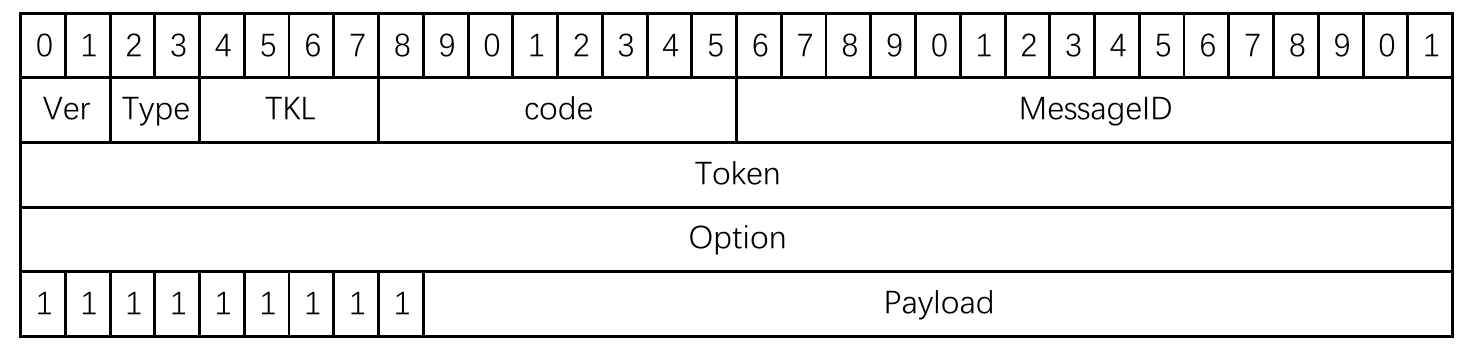
\includegraphics[width=14cm]{CoAP报文.png}
	\caption{CoAP的消息格式}
	\label{CoAP报文}
\end{figure}

  
\begin{table}[h!]
\caption{CoAP字段}
\begin{tabular}{ccc}
\toprule
字段名 & 比特数 & 解释\\
\midrule
Ver&2&代表协议版本,目前为 0x01 \\
Type&2&\makecell[c]{消息类型,CON为可靠传输,需要响应,响应消息类\\型为 ACK 和 RSTNON 为不可靠传输,不需要响应}\\
TKL&4&Token 的长度,目前为 0~8B \\ 
Code&8&	\\
MessageID&16&消息ID,用于标记重发消息\\
Token&&可选,长度为TKL,用于消息安全性或对应一个请求和响应\\
\bottomrule
\end{tabular}
\label{coap字段}
\end{table}


\subsection{MQTT}

MQTT是一种发布/订阅传输协议,基于TCP/IP协议栈构建,具有低开销,低带宽占用的优点,协议中有三种身份:publisher、broker和subcriber,broker起到解耦合的作用。MQTT提供三种消息传递的服务质量水平:

Qos 0 代表消息至多会传输一次,因为NBIOT底层依赖于不可靠的UDP传输,所以会发生消息的丢失。

Qos 1 代表消息至少会传输一次,但因为重发机制可能会导致消息重复。

Qos 2 代表q确保消息会到达一次,保证不会出现消息丢或重复的现象,适用于非幂等的请求传输。

%\begin{table}[h!]
%\caption{MQTT服务质量}
%\begin{tabular}{cc}
%\toprule
%值 & 解释 \\
%\midrule
%Qos 0 & 至多一次 \\
%Qos & 至少一次 \\
%Qos & 只有一次 \\
%\bottomrule
%\end{tabular}
%\label{tablea}
%\end{table}



\begin{figure}[h]
	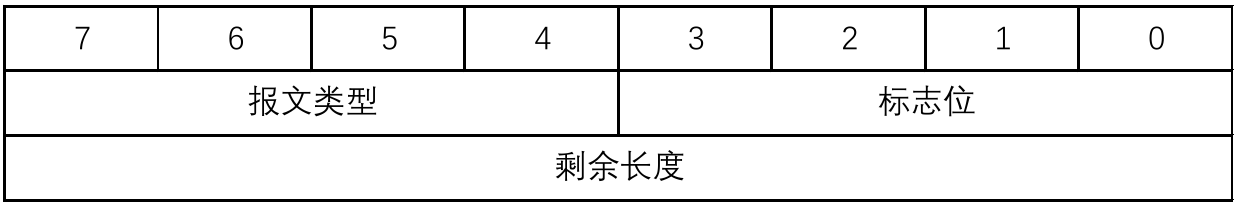
\includegraphics[width=12cm]{MQTT报文.png}
	\caption{MQTT报文结构}
	\label{MQTT报文}
\end{figure}

\begin{table}[h!]
\caption{MQTT报文字段}
\begin{tabular}{ccl}
\toprule
字段名 & 比特数 & 解释\\
\midrule
Control Packet type	&4&控制报文类型,4位无符号数\\
Flags	&4&	\\
Remaining Length&&\makecell[c]{剩余长度表示当前报文余下的负载数据长度\\(不包含自身),使用Base 128 Varints编码}\\
\bottomrule
\end{tabular}
\label{mqtt字段}
\end{table}

\subsection{CoAP和MQTT的异同}


  MQTT协议使用发布/订阅模型,CoAP协议使用请求/响应模型;

  MQTT会通过网关在客户机之间创建连接,CoAP协议则是无连接协议;

  MQTT通过中间代理传递消息的多对多协议,CoAP协议是Server和Client之间消息传递的单对单协议;
  
  MQTT不支持带有类型或者其它帮助Clients理解的标签消息,CoAP内置内容协商和发现支持,允许设备彼此窥测以找到交换数据的方式。


\section{本章小结}

\chapter{NB-IOT通信模块设计}
\section{模块总体介绍}

上海移远通信技术有限公司开发的bc35G通信模组支持 band8、band5、band20、band28频段,采用LCC贴片封装,尺寸为19.9mm*23.6mm*2.2mm,完全符合欧盟RoHs标准\cite{RoHs},外部参数如下:

\begin{table}[h!]
\caption{模块参数}
\begin{tabular}{ll}
\toprule
参数&说明\\
\midrule
供电&3.1V~4.2V,典型电压3.6V\\
省电&PSM模式下最大耗流 5uA\\
发射功率&23dBm +- 2dB\\
温度范围&正常工作温度: -35‘c~+75'C\\
\bottomrule
\end{tabular}
\label{模块参数}
\end{table}

模块的主要部分包括射频前端、电源管理、基带芯片。

射频前端主要包括功率放大器、滤波器,用于无线电信号和二进制信号的互相转换。

基带芯片则是用于信号处理,bc35G模块使用的是华为bionic系列芯片。


\section{供电}
电源是模块稳定运行的基础,对模块的性能以及使用寿命都有显著影响。同时由于NBIOT设备一般需要支持10年的正常使用,稳定可靠的电源也是重中之重。

锂亚电池电池由于其特殊的化学性质和钝化效应,储存寿命达到十年以上,被广泛运用与电子水表和电表等终端设备中作为电源,符合NBIOT应用的一般使用场景。同时其标称电压3.6V,与模块典型电压一致,所以锂亚电池
非常适合用于模块供电。

由于电源电压输出并不是理想直流输出,一般含有交流成分,比如惠州亿纬公司生产的AA型锂亚电池\cite{锂亚电池},在25°C的条件下,未放过电的电池在放电过程中每2分钟会释放一个150mA/0.1秒的脉冲,
所以在电源输入端并联了并联一个100uF的钽电容C1,以及100nF(C2)、100pF(C3)和22pF(C4)的滤波电容。

在模块开机或者电源接入时,一般会产生电涌,其对电子设备损害极大,所以为了避免电涌对模块的损害,在电源输入端增加一个TVS管(D1)以提高模块对浪涌电压的承受能力。

除了遵守一般的嵌入式模块电源设计要求,由于RF天线信号可能在电路中产生感应电流,所以通信模块的电源设计也要考虑到其与无线信号的相互干扰,简单的做法是在PCB布局上使VBAT电源线原理RF天线。

依据上述设计要求,输入端参考电路如图\ref{VBAT}。同时,根据模块的引脚定义表\ref{VBAT引脚定义},选用2脚和45脚作为电源输入的VBAT和GND。
\begin{figure}[H]
	\centering
	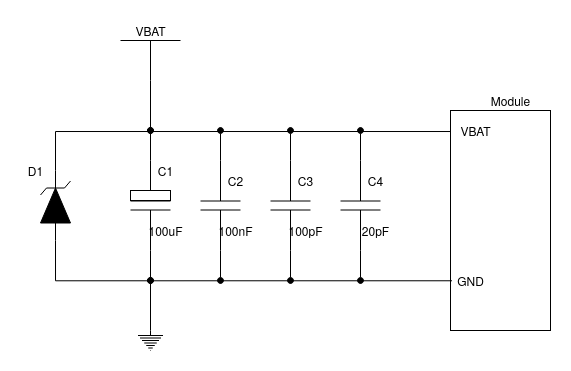
\includegraphics[width=10cm]{VBAT.png}
	\caption{VBAT}
	\label{VBAT}
\end{figure}

\begin{table}[h!]
\caption{VBAT引脚定义}
\begin{tabular}{lllll}
\toprule
  引脚名 & 引脚号 & 最小值 & 典型值 & 最大值\\
 \hline
 VBAT & 45,46 & 3.1V & 3.6V & 4.2V \\
 GND  & 2,43,47,48,51,52,54,59~66,71~74,81~83,92~94 & & 0 & \\
\bottomrule
\end{tabular}
\label{VBAT引脚定义}
\end{table}

\section{省电技术}

NBIOT技术的使用场景一般对设备不更换电源持续使用时间都有较苛刻的要求,比如10年的稳定工作。所以省电技术的支持就十分重要。

对于受限的物联网设备,省电技术一般有3种,分别是DRX(Discontinuous Reception),eDRX(extended DRX),PSM(Power Saving Mode),其基本思想是让通信设备终端周期性进入休眠模式,
在休眠期间不接受物理层消息,关闭收发的射频模块,从而达到省电目的。不同的省电技术一般可以通过不同的软件配置实现,在NBIOT物联网应用开发时,需要根据不同的使用场景使用不同的配置,使模
块能耗降到最低。

DRX技术是指一个周期内拥有两种工作状态,分别是激活态和休眠状态,仅在激活态时进行数据的接收、发送与处理,周期定时器一般可以通过核心网在设备入网时配置,一般配置为0.64s,1.28s,2.56s和
5.12s四种时间,当配置为0.64s时基本可以认为下行消息随时可以送达终端设备,实时性和延迟性能在三种技术中最好,但能耗消耗最大,所以一般用于对时延要求极高或者有稳定供电的场景,比如路灯的开关
应用。DRX模式的示意图如图\ref{drx模式}
\begin{figure}[H]
	\centering
	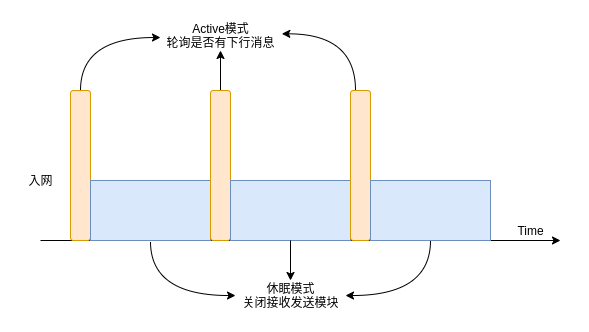
\includegraphics[width=10cm]{drx模式.png}
	\caption{drx模式}
	\label{drx模式}
\end{figure}

eDRX(扩展drx)技术在3GPP Release13中引入。一个eDRX周期相当与多个drx周期的组合,并且区分开接收下行消息和接收寻呼消息的周期。一个激活时间段和一个休眠时间段都
包含多个drx周期,并且激活周期和休眠周期各自包含一个PTW周期,激活周期中的PTW周期可以用于接收下行消息和寻呼消息,激活周期的PTW周期最大支持10.24s。休眠周期则不可以接受下行消息,只能接收寻呼消息,
休眠周期的PTW可以达到40分钟。在休眠周期是也可以通过寻呼消息唤醒终端设备从而接收下行消息,所以也可以认为消息可以时刻到达终端设备,由此可见eDRX技术对延时和能耗有一定的满足。eDRX模式的切换状态
如图\ref{eDRX模式}

\begin{figure}[H]
	\centering
	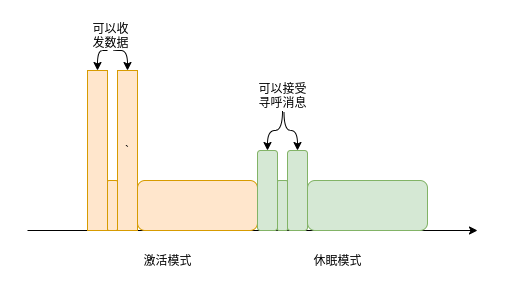
\includegraphics[width=10cm]{eDRX模式.png}
	\caption{eDRX模式}
	\label{eDRX模式}
\end{figure}

PSM模式则是对能耗有极致的要求,放弃了实时性,允许通信模块在PSM模式下完全不可达,所有耗电模块全部关闭。PSM模式的状态切换如图\ref{工作模式切换}。模块需要进入PSM模式,需要先通过 AT+PSM=1 开启模块PSM功能,
在模块入网或进行TAU操作时,将会请求进入PSM模式,得到核心网下发的T3324定时器数值,模块将会休眠直到T3324定时器过期或者模块主动发送消息,在休眠期间除了T3342时钟,所有模块都会关机。PSM模式如图\ref{PSM模式}

\begin{figure}[H]
	\centering
	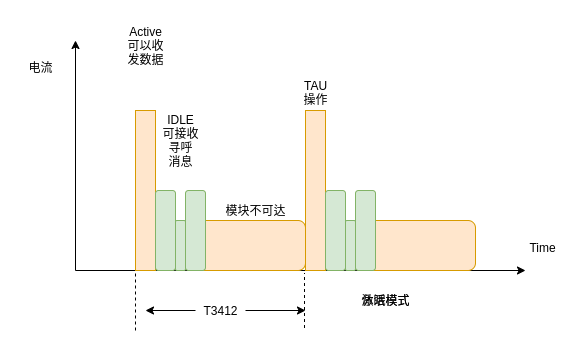
\includegraphics[width=10cm]{PSM模式.png}
	\caption{PSM模式}
	\label{PSM模式}
\end{figure}

模块在各种模式运行情况下,消耗电流如表\ref{消耗电流}

\begin{table}[h!]
\caption{消耗电流}
\begin{tabular}{llll}
\toprule
  模式 & 描述 & 典型值 & 最大值\\
 \hline
 PSM & 睡眠状态 & 3mA & 5mA \\
 IDLE  & 空闲状态 & 2mA & \\
 \multirow{3}{*}{Active} & 射频发射状态(23dBm)(B5/B8/B20) & 230mA & \\
 & 射频发射状态(23dBm)(B28) & 250mA & \\
 & 射频接收状态 & 61mA & \\
\bottomrule
\end{tabular}
\label{消耗电流}
\end{table}

\section{串口}
bc35g模块提供两对串口,分别为主串口和调试串口。主串口用于AT命令的通信、数据传输和固件升级,波特率为9600bps,在Active、Idle和PSM模式下均可工作,调试串口可以通过UE Log Viewer工具查看日志信息,波特率为921600bps。对于串口与上位机的连接,采用传统的DCE-DTE
(date terminal/control equivement)方式连接,模块作为DCE,连接方式如图\ref{DCT-DTE连接}

\begin{figure}[H]
	\centering
	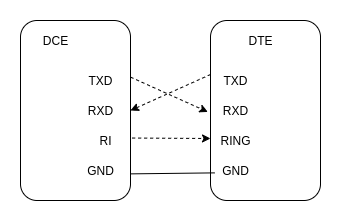
\includegraphics[width=10cm]{DCT-DTE连接.png}
	\caption{DCT-DTE连接}
	\label{DCT-DTE连接}
\end{figure}

RS232作为通用串行总线通信标准,在1970年有美国电子工业协会联合贝尔系统及一些终端生产厂家共同制定,用于DTE-DCE之间的通信,主要作用是将MCU输出的TTL电平转换成RS232电平。TTL电平是指在输出电路上电压大于等于2.4V为逻辑1,电压小于0.4V为逻辑
0,而在输入电路上,电压大于等于2.0v为逻辑1,电压小于等于0.8V为逻辑0。而RS232电平规定-15V 到 -3V代表逻辑1,+3V 到 +15V代表逻辑0。为了使模块能够接入PC调试,需要在MCU引出的串口引脚与PC连接之间加上RS232电平
转换芯片,并且为了降低串口功耗,在电路中加入1k欧姆电阻降低串口电流,RS232转换电路如图\ref{RS232连接图}

\begin{figure}[H]
	\centering
	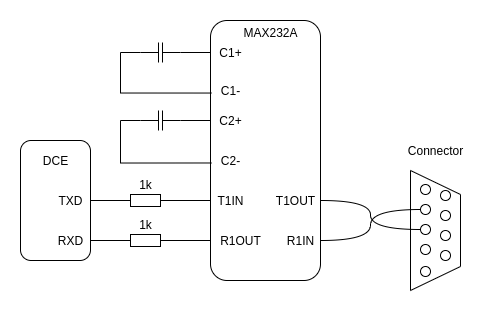
\includegraphics[width=10cm]{RS232连接图.png}
	\caption{RS232连接图}
	\label{RS232连接图}
\end{figure}

\section{射频天线}
BC35G天线部分预留了pi型匹配电路如图\ref{ANT},以便对天线性能调节。C1和C2两个电容将大多数交流成分滤除,R1为0欧电阻,充当pi型RC滤波电路的电感。为了确保射频信号的性能以及可靠性,需要遵循pi型匹配电路的layout。既要保证电容电感布局靠近,也要防止出现stub\cite{OKgagaga,stubeffect}
\begin{figure}[H]
	\centering
	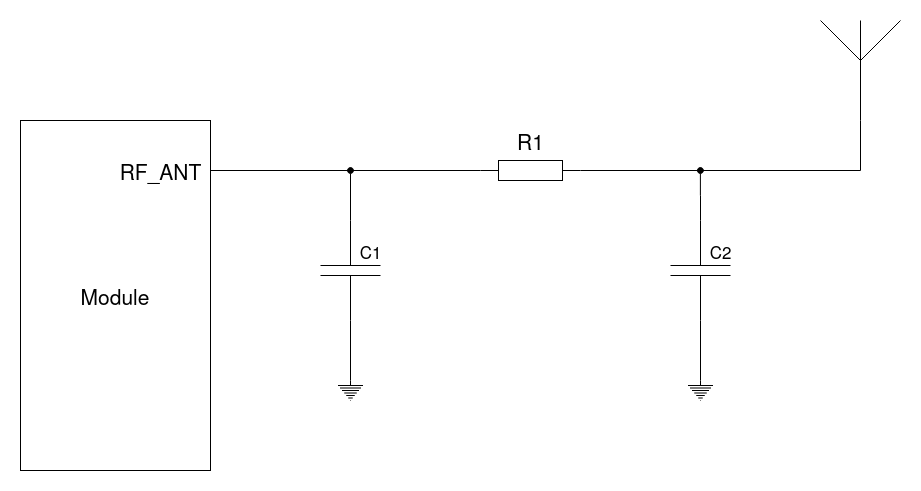
\includegraphics[width=10cm]{ANT.png}
	\caption{ANT}
	\label{ANT}
\end{figure}

对于模块的射频信号线,需要保证PCB上所有射频信号线的特性阻抗控制在50欧姆,控制射频信号新特性阻抗一般采取微带线和共面波导的设计方式,通过控制射频信号线材料的介电常数,地平面参考高度(H),离地间隙(S)以及走线宽度(W),从而改变射频信号线的特性阻抗。

微带线是指在介质基片上由单一的导体带构成的微波传输线,其特点是体积小、重量轻、可用频段宽、可靠性高、制造成本低,但损耗比较大,功率范围比较窄,微带线的结构示意图如图\ref{微带线}

\begin{figure}[H]
	\centering
	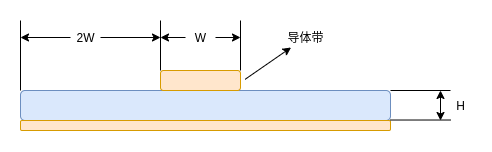
\includegraphics[width=10cm]{微带线.png}
	\caption{微带线}
	\label{微带线}
\end{figure}

共面波导是指在一个面上由两个导体平面夹着一个中心导体带的结构,其相比于微带线,具有工艺简单、屏蔽性能好,接地电感低等优点,但是其衰减损耗更大,导热能力也不理想,导致不适用于大功率的放大器。两层共面波导的结构示意图如\ref{共面波导}

\begin{figure}[H]
	\centering
	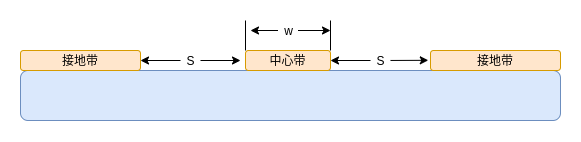
\includegraphics[width=10cm]{共面波导.png}
	\caption{共面波导}
	\label{共面波导}
\end{figure}

在实际的电路设计中,为了确保射频信号的性能和可靠性能够满足要求,在电路模拟时需要精确地控制射频信号线的阻抗为50欧姆,射频引脚到天线连接器之间的走线避免走90度角,情况允许尽量走135度角。与射频引脚相连的GND引脚也不做热焊盘,要与地充分接触。

\section{USIM卡座}
USIM全称为Universal Subscriber Identity Module,是SIM卡(Subscriber Identity Module)的升级。USIM卡是一个内置有MCU的芯片卡,内部包含一个
位CPU,一个3到8kbit的程序存储器(ROM),一个6到16kbit的工作存储器(RAM),一个128到256kbit的数据存储器(EEPROM)和串行通信单元5个模块,需要5个引脚才能正常工作,
分别是电源VDD,时钟CLK,数据IO Data,复位 RST,接地 GND,引脚的定义及功能如表\ref{USIM引脚定义}

\begin{table}[h!]
\caption{USIM引脚定义}
\begin{tabular}{lll}
\toprule
  引脚名称 & 引脚号 & 描述 \\
 USIM\_VDD & 38 & 外部USIM卡供电电源,电压3.0v \\
 USIM\_CLK  & 41  & 外部USIM卡时钟线  \\
 USIM\_DATA & 40 & 外部USIM卡数据线  \\
 USIM\_RST & 39 &  外部USIM卡复位线  \\
 USIM\_GND & 42 & 外部USIM卡转用地  \\
\bottomrule
\end{tabular}
\label{USIM引脚定义}
\end{table}

支持3GPP规范功能的USIM卡使模块能够接入运营商网络,USIM功能包括模块和卡座,为了确保USIM卡的性能以及避免与射频、电源模块的干扰,须遵循以下设计原则:

\begin{enumerate}
\item USIM卡座和模块尽量靠近摆放,尽量保证USIM信号线布线长度不超过200mm保证信号品质
\item 外部USIM信号线布线应尽量远离射频线号线走线及电源VBAT走线
\item 防止USIM\_DATA和USIM\_CLK信号干扰,两线之间加入地屏蔽,并保持一定的距离。在USIM\_RST信号也需要地保护
\item USIM\_DATA, USIM\_VDD, USIM\_CLK, 和USIM\_RST并联33pF电容滤除射频线号线的的干扰
\item 为了防止静电,在卡座和模块之间增加TVS管,TVS管的寄生电容应不大于55pF
\end{enumerate}


USIM卡座电路图如\ref{USIM}
\begin{figure}[H]
	\centering
	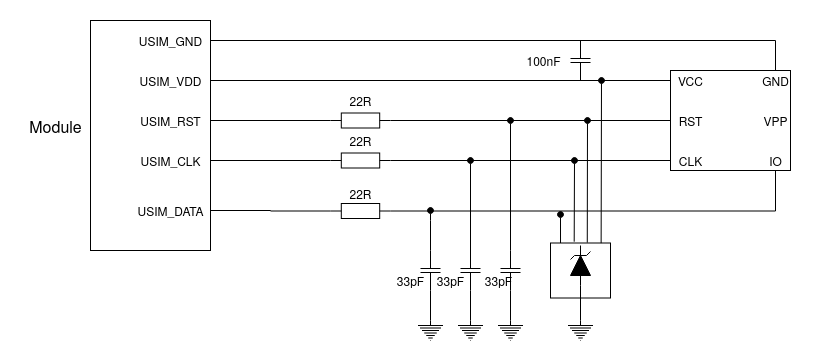
\includegraphics[width=10cm]{USIM.png}
	\caption{USIM}
	\label{USIM}
\end{figure}

\section{本章小结}

本章讨论了BC35G模块的外围电路设计,包括USIM卡座、电源、天线以及串口,主要关注于各部分之间的信号干扰避免,通过合理使用滤波电容,不同部分在电路板上的位置的相对远离,以达到良好的射频信号性能以及可靠性。同时通过TVS管等方式降低电涌对设备的损害。


\lstset{
 columns=fixed,       
 numbers=left,                                        % 在左侧显示行号
 numberstyle=\tiny\color{gray},                       % 设定行号格式
 frame=none,                                          % 不显示背景边框
 backgroundcolor=\color[RGB]{245,245,244},            % 设定背景颜色
 keywordstyle=\color[RGB]{40,40,255},                 % 设定关键字颜色
 numberstyle=\footnotesize\color{darkgray},           
 commentstyle=\it\color[RGB]{0,96,96},                % 设置代码注释的格式
 stringstyle=\rmfamily\slshape\color[RGB]{128,0,0},   % 设置字符串格式
 showstringspaces=false,                              % 不显示字符串中的空格
 language=c,                                        % 设置语言
}


\chapter{模块验证与实验}
基于NB-IOT的中断应用大致分为4类,分别是固定上报类,固定控制类,移动上报类和移动控制类。不同类别的应用因为数据的实时性、数据量、部署环境等的不同,对网络以及电源的需求也不同。例如对于固定控制类,由于设备部署位置固定,常有外部电源支持,需要较强的实时性,所以对功耗需求不高,需要模块时刻保持在线状态。接下来将以一个固定上报类终端对bc35g模块进行验证。
\section{华为云平台应用开发}
华为 OceanConnect物联网平台作为一个连接业务应用和物联网设备的中间层,提供了海量设备接入管理,屏蔽复杂的设备接口,可以快速构筑物联网应用。
%\begin{figure}[h]
%    \floatcontinue
%	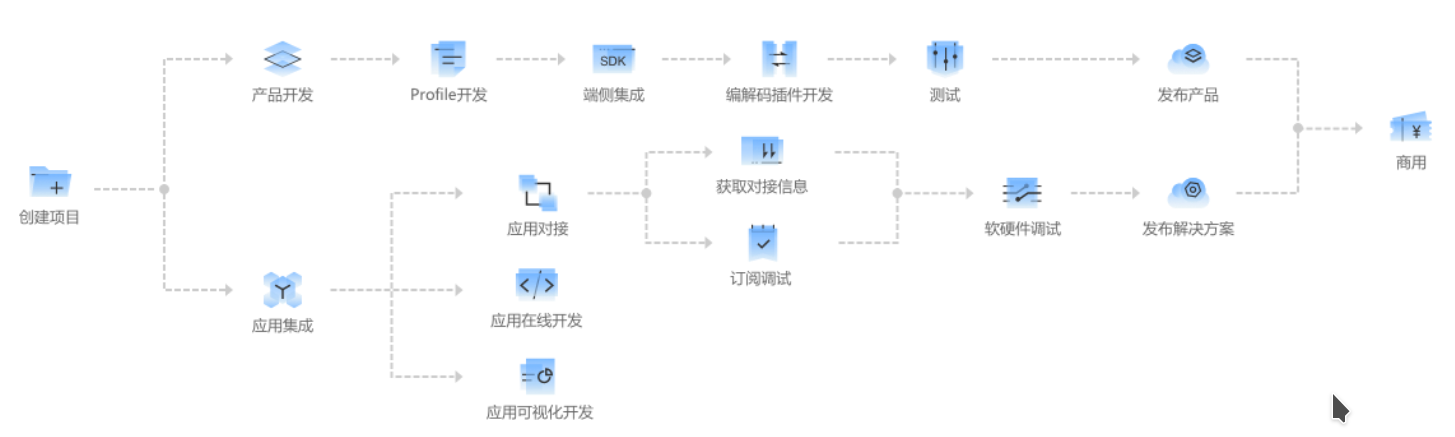
\includegraphics[width=20cm]{oc流程.png}
%	\caption{oc流程}
%	\label{oc流程}
%\end{figure}

\subsection{定义产品}
产品是指一类具备相同能力和特征的设备,一个产品包含产品模型、编解码插件等资源。选用CoAp协议,由于使用JSON的数据格式对能耗消耗太大,不适用于物联网设备,所以选用二进制码流的数据格式,通过开发编解码插件解析。
\begin{figure}[H]
    \centering
	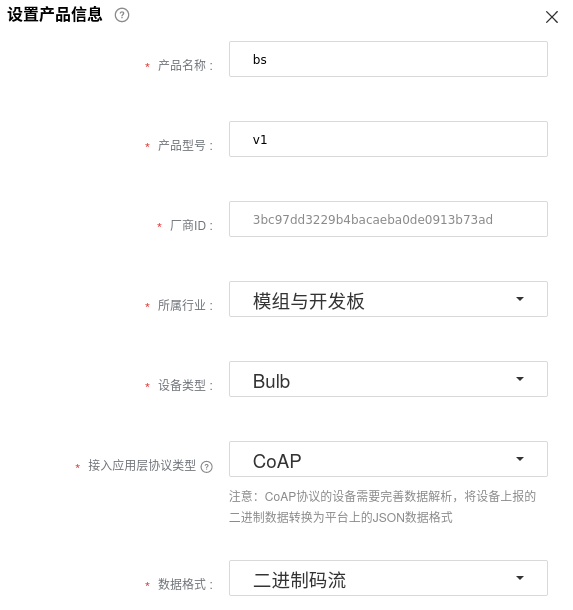
\includegraphics[width=9cm]{oc产品.png}
	\caption{oc产品定义}
	\label{oc产品}
\end{figure}


\subsection{定义profile与编解码插件}
profile是描述产品设备信息的文件,定义了设备与应用服务器交互的字段及格式。其主要包含产品信息、服务能力以及维护能力。以控制开发板LED灯相关的profile信息为例,定义profile如下:
\begin{table}[h]
\caption{profile格式}
\begin{tabular}{|c|c|c|c|c|}
\toprule
\multicolumn{5}{|l|}{属性列表} \\
\hline
属性名称 & 类型 & 取值 & \multicolumn{2}{|c|}{描述}  \\
\hline
status & int & 0~1 & \multicolumn{2}{|l|}{0:灯关闭 1:灯开启} \\
\toprule
\multicolumn{5}{|l|}{命令列表} \\
\hline\
命令名称 & 字段属性 & 字段名 & 取值 & 描述\\
\hline
\multirow{3}{*}{led} & 请求 & num & 1-2 & led 编号 \\
\cmidrule{2-5}
                     & 请求 & status & 0-1 & led状态 \\
\cmidrule{2-5}
                     & 响应 & result & 0-1 & 执行命令结果 \\
\hline
\multirow{2}{*}{beep} & 请求 & status & 0-1 & 蜂鸣器状态 \\
\cmidrule{2-5}
                      & 响应 & result & 0-1 & 执行命令结果 \\
\hline
\multirow{2}{*}{query} & 请求 & resource & 1-3 & 资源编号 \\
\cmidrule{2-5}
                      & 响应 & result & 0-1 & 执行命令结果 \\
\bottomrule
\end{tabular}
\label{tablea}
\end{table}

二进制数据格式需要编解码插件才能解析,在oc平台上设置好profile 文件后,将相应属性值与消息模板中的字段相连接,oc平台将会自动生成编解码器。

\subsection{接入设备}
通过串口连接设备,使用AT+CSGB=1命令查询设备IMEI号,在oc平台上增加设备,并从oc平台获取CoAP接入地址,填入stm32代码,华为云平台上的设置就完成了。(TODO:补图)


\section{stm32终端开发}
stm32终端选择一块搭载stm32f103zet的开发板,板载4组串口,第一组可用于USB通信。本次验证使用到其中第二组串口,对应引脚为PA2和PA3。使用无源蜂鸣器及一组LED灯,作为控制量,对应引脚为PB8,PB5,PE5。


\subsection{串口DMA通信}

stm32开发板控制bc35g模块是通过串口的方式,bc35g串口比特率为9600。由于HAL库函数仅提供接受固定长度数据的封装,为了接受变长的串口数据,可以有以下几种方式:

BC35G模块串口传输数据以'lr cr'为分隔符,以软件的方式,设置超时接收固定长度并以'lr cr'分割,放入缓冲区中。由于模块涉及网络操作等原因,不同AT指令的响应时间有很大差距,所以超时时间不好确定,同时由于MCU等待模块输入,对效率影响较大。

利用定时器中断方式可以超时时间设置的问题。一个字节的数据有 起始位+数据+结束位共10位,在模块串口比特率为9600的情况下,传输一个字节需要104us。同时由于两组数据之间需要间隔3.5字符,可以设置定时器中断为5ms。在串口接受中断服务函数中开启定时器中断,每接受一个字符则重置定时器,当定时器超时时可以认为一组数据接受完毕,在定时器中断函数中将接收到的数据放入缓存中。但是由于是一字节一字节接受,而且MCU仍然参与接受过程,所以效率仍有提升必要。

为了进一步提升效率,可以使用DMA方式接受数据。为了区分两组数据,开启总线空闲中断,在总线空闲中断中标记数据就绪。这种方式能获得更好的效率。

\begin{lstlisting}

/* main.c
* 使能串口2的总线空闲中断
*/
__HAL_UART_ENABLE_IT(&huart2,UART_IT_IDLE);

/* uart.c
* 检测空闲中断,标记数据可用,并重新开启中断用于下次接收
*/

uint8_t UART2DATAREADY = 0;
uint8_t UART2RXBUFFER[UART_BUFFER_SIZE];

void USER_UART_IRQHandler(UART_HandleTypeDef *huart) {
    if (huart == &huart2) {
        if (RESET != __HAL_UART_GET_FLAG(&huart2, 
                UART_FLAG_IDLE)) {
            __HAL_UART_CLEAR_IDLEFLAG(&huart2);
            HAL_UART_DMAStop(&huart2);
            UART2DATAREADY = UART_BUFFER_SIZE - 
            __HAL_DMA_GET_COUNTER(&hdma_usart2_rx);
        }
    }
}

/* nbiot.c
* 封装AT指令执行模块,接收串口回传数据
*/
void NBCommand(uint8_t *com, uint8_t com_size, 
                char *res, uint8_t *res_size) {
    HAL_UART_Transmit(&huart2, com, com_size - 1, 0xfff);
    HAL_UART_Receive_DMA(&huart2, 
                        UART2RXBUFFER, 
                        UART_BUFFER_SIZE);
    while (!UART2DATAREADY) {
        HAL_Delay(50);
    }
    memcpy(res, UART2RXBUFFER, UART2DATAREADY);
    *res_size = UART2DATAREADY;
    UART2DATAREADY = 0;
}

\end{lstlisting}

\subsection{入网初始化}
bc35g模块入网操作流程如图(TODO:临时图)

\begin{figure}[H]
    \centering
	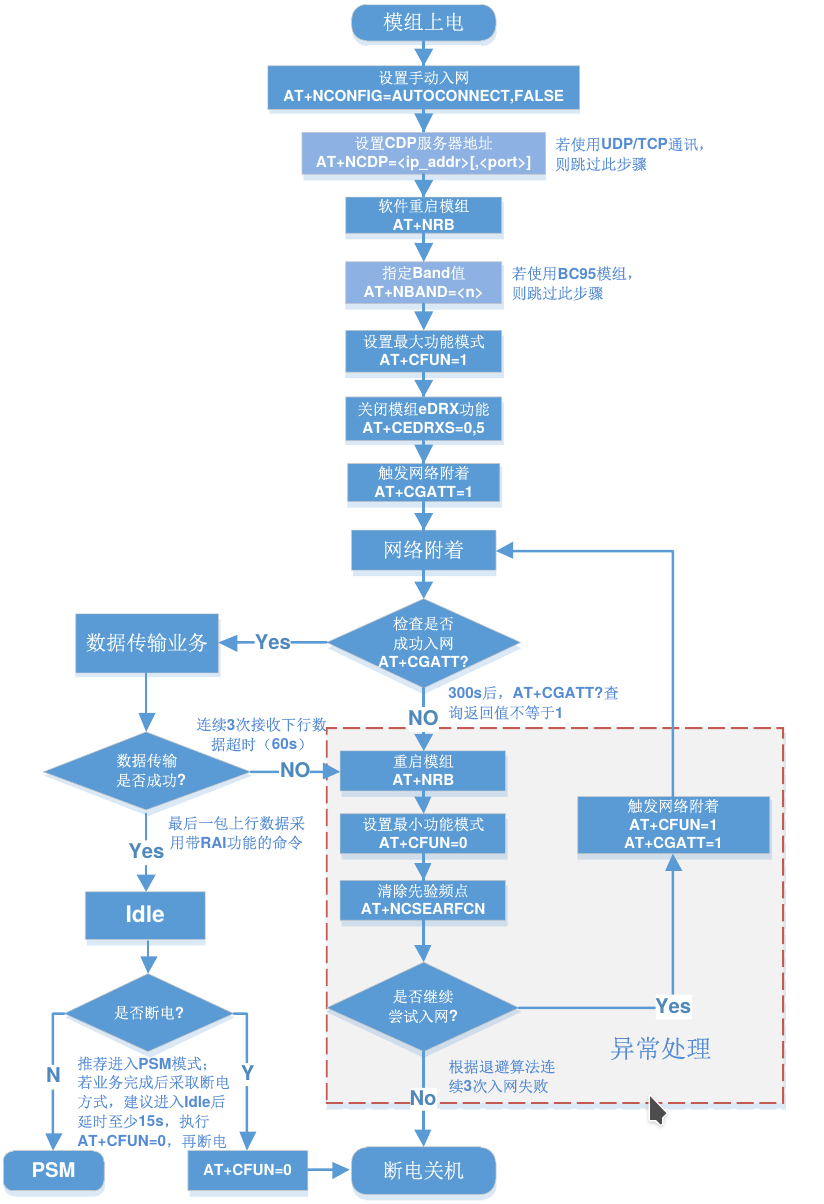
\includegraphics[width=10cm]{模块入网操作.png}
	\caption{模块入网}
	\label{模块入网}
\end{figure}

\begin{lstlisting}

/*
* nbiot.c
*/
uint8_t (*InitProc[])() ={
        __NB_MODULE_STATUS,
        __NB_SIGNAL_QUALITY,
        __NB_Manual,
        __NB_SetCDP,
        __NB_ModReboot,
        __NB_SetBand,
        __NB_SetBand,
        __NB_OpenCFun,
        __NB_EdrxOff,
        __NB_PSMOff,
        __NB_NETATT,
};

uint8_t NBInit() {
    unsigned int it = 0;
    for (it = 0; it < sizeof InitProc; it++) {
        if (!InitProc[it]()) {
            NBERROR(it);
        }
    }
    return 1;
}
\end{lstlisting}

\subsection{模组通信}

NBIOT模块使用 AT+NMGS命令发送数据

\subsection{退网关机}
\begin{lstlisting}

\end{lstlisting}


\section{验证过程以及结论}

\section{本章小结}

\chapter{全文总结与展望}

\section{全文总结}
(temp-TODO:代码地址 https://github.com/chilogen/stm32\_test/tree/feature/nbiot-bs)

(temp-TODO:论文地址 https://github.com/chilogen/ThesisUESTC)


\section{后续工作展望}

模块的实际设计与开发需要投入不少资源用于生产试错的过程,就如FPGA的出现为芯片设计提供了极大地便利一样,SDR(Software Defined Radio)通过软件来模拟传统的硬连线方式实现无线电通信,只需使用不同的软件就能在通用PC上实现一个通信模块具有的功能,不仅方便了无线电爱好者低成本的探索无线电世界,对于通信协议的研究也提供了快捷的方式。预期通过对通信原理的深入学习,可以实现用于gnuradio的NB-IOT插件,更加方便对NB-IOT技术的学习。
%\chapter{template}
This is the template of the chapter in split file.

\section{s1}
This is a section.

\subsection{sub1}
This is a subsection.


%
%%[1] 王浩刚,聂在平.三维矢量散射积分方程中奇异性分析[J].电子学报,1999, 27(12): 68-71
%
%@article{wang1999sanwei,
%  title = {三维矢量散射积分方程中奇异性分析},
%  author = {王浩刚 and 聂在平},
%  journal = {电子学报},
%  volume = {27},
%  number = {12},
%  pages = {68--71},
%  year = {1999}
%}
%
%%[2] X. F. Liu, B. Z. Wang, W. Shao. A marching-on-in-order scheme for exact attenuation constant extraction of lossy transmission lines[C]. China-Japan Joint Microwave Conference Proceedings, Chengdu, 2006, 527-529
%
%@conference{liuxf2006,
%  author = {Liu, X F and Wang, Bing Zhong and Shao,Wei and Wen Wang},
%  title = {A marching-on-in-order scheme for exact attenuation constant extraction of lossy transmission lines},
%  year = {2006},
%  pages = {527-529},
%  address = {Chengdu},
%  booktitle = {China-Japan Joint Microwave Conference Proceedings}
%}
%
%%[3] 竺可桢.物理学[M].北京:科学出版社,1973, 56-60
%
%@book{zhu1973wulixue,
%  title = {物理学},
%  author = {竺可桢},
%  year = {1973},
%  address = {北京},
%  pages = {56-60},
%  publisher = {科学出版社}
%}
%
%%[4] 陈念永.毫米波细胞生物效应及抗肿瘤研究[D].成都:电子科技大学,2001, 50-60
%
%@thesis{chen2001hao,
%  author = {陈念永},
%  title = {毫米波细胞生物效应及抗肿瘤研究},
%  institution = {电子科技大学},
%  year = {2001},
%  pages = {50-60},
%  address = {成都}
%}
%
%%[5] 顾春.牢牢把握稳中求进的总基调[N].人民日报,2012年3月31日
%
%@newspaper{gu2012lao,
%  author = {顾春},
%  title = {牢牢把握稳中求进的总基调},
%  journal = {人民日报},
%  date = {2012年3月31日}
%}
%
%%[6] 冯西桥.核反应堆压力容器的LBB分析[R].北京:清华大学核能技术设计研究院,1997年6月25日
%
%@techreport{feng997he,
%  author = {冯西桥},
%  title = {核反应堆压力容器的{LBB}分析},
%  institution = {清华大学核能技术设计研究院},
%  date = {1997年6月25日},
%  address = {北京}
%}
%
%%[7] 肖珍新.一种新型排渣阀调节降温装置[P].中国,实用新型专利,ZL201120085830.0, 2012年4月25日
%
%@patent{xiao2012yi,
%  author = {肖珍新},
%  title = {一种新型排渣阀调节降温装置},
%  date = {2012年4月25日},
%  type = {实用新型专利},
%  country = {中国},
%  id = {ZL201120085830.0}
%}
%
%%[8] 中华人民共和国国家技术监督局.GB3100-3102.中华人民共和国国家标准--量与单位[S]. 北京:中国标准出版社,1994年11月1日
%
%@standard{zhong1994zhong,
%  institution = {中华人民共和国国家技术监督局},
%  id = {GB3100-3102},
%  title = {中华人民共和国国家标准--量与单位},
%  publisher = {中国标准出版社},
%  date = {1994年11月1日},
%  address = {北京}
%}
%
%@digital{clerc2010discrete,
%  author = {M. Clerc},
%  title = {Discrete particle swarm optimization: a fuzzy combinatorial box},
%  type = {EB/OL},
%  date = {July 16, 2010},
%  url = {http://clere.maurice.free.fr/pso/Fuzzy_Discrere_PSO/Fuzzy_DPSO.htm}
%}

% misc

\thesisacknowledgement

非常感谢鲁晓军老师在毕设期间提供的悉心指导和检查老师认真负责提出的修改意见。

\thesisappendix

\chapter{abc}

\section{abc}

\nocite{*}
\thesisbibliography{reference}

%
% Uncomment the following code to load bibliography database with native
% \bibliography command.
%
% \nocite{*}
% \bibliographystyle{thesis-uestc}
% \bibliography{reference}
%

\thesisaccomplish{publications}
\input{misc/translate_original}
\input{misc/translate_chinese}

\end{document}
